\documentclass[manuscript,screen,review]{acmart}

\settopmatter{printacmref=true}
\setcopyright{rightsretained}
\acmJournal{TCPS}
\copyrightyear{2026}

\usepackage{booktabs}
\usepackage{tabularx}
\usepackage{array}
\usepackage{amsmath}
\usepackage{graphicx}
\usepackage{algorithm}
\usepackage{algpseudocode}
\usepackage{seqsplit}
\usepackage{url}

\Urlmuskip=0mu plus 1mu
\emergencystretch=3em

\newcommand{\SCAA}{SCAA-PLC}

\begin{document}

\title{SCAA-PLC: A Boundary-Aware Evidence-Card Method for PLC Binary Analysis}

\author{Bowei Ning}
\email{2020183@stu.syuct.edu.cn}
\orcid{0000-0003-4553-9096}
\affiliation{%
	\department{School of Artificial Intelligence}
	\institution{Shenyang University of Technology}
	\city{Shenyang}
	\country{China}
}
\affiliation{%
	\institution{Key Laboratory of Information Security for Petrochemical Industry in Liaoning Province}
	\city{Shenyang}
	\country{China}
}

\author{Xuejun Zong}
\authornote{Corresponding author.}
\email{xuejun\_zong@syuct.edu.cn}
\orcid{0009-0000-0084-2775}
\author{Lian Lian}
\authornote{Corresponding author.}
\email{lianlian@syuct.edu.cn}
\orcid{0000-0002-5093-2450}
\author{Kan He}
\email{hekan1978@syuct.edu.cn}
\author{Yifei Sun}
\email{sunyifei@syuct.edu.cn}
\author{Yuxiang Lei}
\email{z2023365@stu.syuct.edu.cn}
\affiliation{%
	\department{School of Information Engineering}
	\institution{Shenyang University of Chemical Technology}
	\city{Shenyang}
	\country{China}
}
\affiliation{%
	\institution{Key Laboratory of Information Security for Petrochemical Industry in Liaoning Province}
	\city{Shenyang}
	\country{China}
}

\author{Plamen Vasilev}
\email{plamen.vasilev@uctm.edu}
\affiliation{%
	\department{Department of Industrial Automation}
	\institution{University of Chemical Technology and Metallurgy}
	\city{Sofia}
	\country{Bulgaria}
}

\renewcommand{\shortauthors}{Ning et al.}

\begin{abstract}
Aggregate metrics in binary-analysis studies do not retain which observations support each sample or why a tool produced no usable output. Symbol-Consistent Auditable Analysis for PLC binaries (SCAA-PLC) is an evidence-card reporting method that joins typed observation slots, uncertainty codes, source rules, hashes, and execution records without treating tool output as semantic ground truth. We construct cards for all 2{,}431 PLC-BEAD binaries and use 1{,}876 rows with an unambiguous Structured Text mapping for source-role analysis. A same-snapshot validity case finds exact agreement for a GEB-scoped naming rule, while its ungated lexical predicate has zero recall on 735 source-positive OpenPLC rows. Three empirical channels and six typed slots retain identical information on the evaluated tasks; the additional slots preserve provenance rather than add measured discrimination. A bounded second-pipeline instantiation joins 10 OpenPLC binaries to 6{,}657 radare2 relation rows and 20 uncertainty records. Across both paths, five machine-checkable invariants verify identity hashes, uncertainty closure, unsupported-sample handling, source traces, and cross-pipeline joins with zero failures. The method therefore guarantees traceable, uncertainty-closed records under the evaluated contracts; human utility, semantic accuracy, and vulnerability-detection effectiveness remain unevaluated.
\end{abstract}

\begin{CCSXML}
<ccs2012>
<concept>
<concept_id>10002978.10003006.10003013</concept_id>
<concept_desc>Security and privacy~Systems security</concept_desc>
<concept_significance>500</concept_significance>
</concept>
</ccs2012>
\end{CCSXML}
\ccsdesc[500]{Security and privacy~Systems security}

\keywords{PLC binaries, empirical software evaluation, evidence cards, provenance, uncertainty logging, reproducibility}

\maketitle


% Source: PAPER1_MANUSCRIPT_S1_INTRODUCTION_DRAFT.md

\section{Introduction}

Empirical binary-analysis studies commonly compress heterogeneous samples into aggregate scores. Such scores cannot show which binary-visible observations were available, whether a result came from binary content or benchmark metadata, or why a tool produced no usable output. This creates a software-evaluation problem: reviewers can inspect the reported metric without being able to trace each sample to its input, transformation, evidence state, and known boundary. SCAA-PLC addresses that problem for PLC binary-analysis studies. It does not evaluate a physical process, operational safety decision, or vulnerability-detection task.

A concrete example illustrates the gap. For \texttt{geb\_ARRAY\_HAV}, GNU \texttt{nm} emits a \texttt{dt\_FB\_} name and the corresponding Structured Text file explicitly declares a \texttt{FUNCTION\_BLOCK}. For \texttt{geb\_AIN}, the source instead declares a \texttt{FUNCTION}; its card records no direct function-block support. For \texttt{codesys\_\_ARRAY\_ABS}, the same \texttt{nm}-based path emits no symbols, so the card records a format/tool boundary rather than a negative semantic finding. An aggregate metric cannot preserve these different evidential states.

The primary study uses all 2{,}431 PLC-BEAD binaries from CODESYS, GEB Automation IDE (GEB), OpenPLC v2, and OpenPLC v3. A deterministic ten-fold assignment keeps samples sharing the same inferred program name in one fold. The historical function-classification task can score 2{,}353 rows, but that label gate no longer controls the present reporting tasks: card and tool-output accounting use all 2{,}431 rows, and source-role analysis uses the 1{,}876 rows with an unambiguous Structured Text mapping. This is an inferred-name-disjoint protocol, not a source-clone-disjoint protocol. The reporting contract retains six typed trace slots, source rules, uncertainty events, graph records, and execution logs. Because four slots co-fill on PLC-BEAD, the evaluation compares a two-field availability summary, a three-channel representation, and the full six-slot record rather than assuming that every slot adds independent information.

The validity design separates a production rule from a transfer probe. SA-001 is explicitly scoped to GEB and agrees with the source-syntax oracle on 353 function-block and 264 non-function-block rows. A separate ungated probe removes only the toolchain gate and applies the unchanged \texttt{dt\_FB\_} pattern to all three source-available toolchains. The probe has zero recall on 359 OpenPLC v2 and 376 OpenPLC v3 source-positive rows. These OpenPLC rows are false negatives for the ungated probe, not for the scoped production rule. Because the pattern and oracle come from one snapshot, this is a post-hoc worked validity case rather than prospective compiler-independent validation.

Two further analyses test the reporting method rather than the GEB convention alone. First, a transparent signature decoder is trained on nine inferred-name folds and evaluated on the tenth. All three schemas preserve the 2{,}431-row binary tool-output boundary exactly. For source-function-block presence, the three-channel and six-slot representations have the same balanced accuracy (0.692) and macro F1 (0.638), compared with 0.500 and 0.367 for the two-field summary. The six slots therefore add provenance detail but no measured discrimination over three channels on PLC-BEAD. Second, an adapter instantiates the same contract over an independently generated native OpenPLC/radare2 evidence set. All 10 binary hashes join to 6{,}657 relation rows and 20 uncertainty records. This is a bounded second-pipeline contract instantiation, not evidence of compiler, vendor, or ecosystem portability.

This paper makes four contributions:

\begin{enumerate}
\item It defines a sample-level evidence-card contract that separates tool observations, claim support, uncertainty, provenance, and execution records, with five machine-checkable invariants and row-level trace cases.
\item It separates a GEB-scoped production rule from an ungated cross-toolchain probe and evaluates the same-snapshot lexical boundary against a separately extracted source-syntax oracle.
\item It evaluates schema complexity through fold-wise information-retention tasks and shows that three empirical channels match the six-slot record on the evaluated tasks, while two fields lose source-role information.
\item It demonstrates bounded record-contract instantiation on a second native OpenPLC/radare2 pipeline and retains hash, relation, and uncertainty boundaries for every adapted card.
\end{enumerate}

These contributions target three research questions:
\begin{itemize}
\item \textbf{RQ1 (Rule validity and transfer):} Does the scoped GEB rule agree with a separately extracted source-syntax oracle, and what happens when its lexical predicate is applied without a toolchain gate?
\item \textbf{RQ2 (Schema economy):} What information is retained by two-field, three-channel, and six-slot evidence-card representations on tool-output and source-role tasks?
\item \textbf{RQ3 (Bounded contract instantiation):} Can the reporting contract be instantiated over a second binary-analysis pipeline while preserving hashes, relation provenance, and explicit uncertainty?
\end{itemize}

Section~2 reviews PLC binary recovery and empirical reporting. Section~3 defines the task-specific populations, evidence sets, and controls. Section~4 specifies SCAA-PLC, Section~5 evaluates rule validity, schema economy, contract invariants, bounded second-pipeline instantiation, and execution controls, and Section~6 discusses interpretation and limitations.


% Source: PAPER1_MANUSCRIPT_S2_BACKGROUND_DRAFT.md

\section{Background and Related Work}

PLC binary analysis sits at the intersection of industrial-control semantics, compiler artifacts, and evaluation design. Operational technology guidance supplies the control-system context~\cite{nist_sp800_82r3}. Firmware systems such as FIRMADYNE, KARONTE, FirmSolo, HALucinator, and SaTC pursue re-hosting, cross-binary analysis, or vulnerability discovery~\cite{firmadyne_ndss2016,karonte_sp2020,firmsolo_usenix2023,halucinator_usenix2020,satc_tdsc2024}; they do not provide a commensurate baseline for sample-level evidence reporting.

Binary representation and symbol-recovery methods illustrate stronger analysis outputs. SAFE and sem2vec learn function representations~\cite{safe_dimva2019,sem2vec_tosem2023}, whereas ReSym reconstructs variable and data-structure names in stripped binaries~\cite{resym_ccs2024}. SCAA-PLC instead records what a configured public-tool path observed and why a field remains unsupported.

The reporting design follows four methodological lines. Benchmark measurements require a specified task, workload, and interpretation~\cite{sim_benchmarking2003}; code duplication can inflate cross-partition evaluation~\cite{allamanis2019adverse}; and computational provenance connects workflow inputs, transformations, and outputs~\cite{freire_provenance2008}. Software-engineering reporting guidelines and later practice studies show both the value of explicit experiment metadata and persistent omissions in published reports~\cite{kitchenham_reporting2008,revoredo_reporting2021}. Metadata-driven experimentation extends that direction toward machine-interpretable study records~\cite{santana_metadata2026}, while artifact studies emphasize persistent, executable research packages~\cite{heumueller_software_artifacts2020}. EUBA explicitly studies uncertainty sources and their presentation to binary analysts~\cite{euba_sandia2021}. Datasheets, Model Cards, and the 2026 Evaluation Cards preprint document datasets, models, and evaluation records at broader levels~\cite{datasheets_for_datasets,model_cards,evaluation_cards_arxiv2026}. SCAA-PLC narrows these ideas to per-sample PLC-binary observations, read provenance, and unsupported-output states. Its novelty is the PLC-binary observation contract rather than a claim to a universal reporting schema, and human analyst benefit remains unevaluated.

\subsection{PLC-BEAD, PLCEmbed, and public PLC binary benchmarks}

PLC-BEAD and PLCEmbed provide the public dataset and reference baseline context~\cite{plcbead_plcembed_kdd2025,plcbead_plcembed_repo}. PLC-BEAD contains CODESYS, GEB, OpenPLC v2, and OpenPLC v3 binaries under a shared label space. PLCEmbed applies a convolutional and Transformer-style raw-byte model and reports 40.35\% function-classification F1 under its original non-program-level split. The local split instead prevents identical inferred program names from crossing folds. The two results therefore require protocol attribution rather than direct ranking.

PLC binary datasets contain compiler variants and source-level relatives. A row-level split can place same-name variants in both partitions. The inferred-name-disjoint split used here prevents that specific overlap but does not identify renamed or near-duplicate source programs. It is therefore an auditable partition condition, not evidence of generalization to all unseen program families.

\subsection{Program-level re-evaluation and protocol context}

PLC-BinX provides the closest external reference for that choice~\cite{plcbinx_arxiv2026}. It reports PLCEmbed function-classification F1 of 4.90\% under a ten-fold program-level re-evaluation, whereas the PLCEmbed KDD 2025 result is 40.35\% under the original split. Their difference demonstrates protocol sensitivity; it does not isolate split policy as the only causal factor, because implementation and aggregation details also differ. One-fold local classifier diagnostics are retained only in the artifact's \path{history/} directory; they are not part of the method contribution, submission supplement, or a reproduction of either published aggregate.

The published results motivate protocol-qualified reporting. Regardless of whether an aggregate score is high or low, it can combine readable symbols, weak state-role support, runtime-only artifacts, and configured-tool gaps. SCAA-PLC therefore adds per-sample evidence and uncertainty records rather than treating unlike protocol values as a leaderboard.

\subsection{CODESYS reverse engineering and format-specific boundaries}

CODESYS is a central configured-tool boundary in PLC-BEAD because the local samples are v3 \texttt{.app} files. ICSREF targets CODESYS v2 \texttt{.PRG} artifacts~\cite{icsref_ndss2019}; the local compatibility audit found Python 2.7, format, header-offset, and architecture-heuristic mismatches. Benkraouda et al. demonstrated that CODESYS-specific format knowledge can enable analysis beyond generic tools~\cite{benkraouda_codesys2023}. These results prevent the local negative \texttt{nm} finding from being generalized to CODESYS binaries as a class.

Rapid7's CODESYS analysis and vendor source-upload documentation further show that engineering artifacts and runtime interactions have format-specific lifecycle assumptions~\cite{rapid7_codesys_whitepaper2023,codesys_source_upload_docs}. Source transfer and engineering-project handling are not equivalent to static recovery of a local \texttt{.app} container. The evidence cards therefore record only that \texttt{nm} emitted no symbols under the evaluated configuration.

This framing avoids treating the CODESYS subset as an error case to be hidden. A transparent result should state which samples are unsupported by the configured tools and why. SCAA-PLC therefore carries CODESYS through the evidence-card pipeline as explicit uncertainty, preserving the distinction between a negative tool-output finding and a positive recovery claim.

\subsection{IEC 61131-3 and declared PLC state-role naming}

IEC 61131-3 defines functions, function blocks, and programs as program organization units (POUs)~\cite{iec61131_3}. This standard supplies the semantic vocabulary for distinguishing a stateful function block from other POU roles. It does not prescribe compiler-emitted binary symbol names. The observed \texttt{dt\_FB\_} prefix is therefore treated as a GEB-specific naming convention found in this dataset, not as an IEC requirement or a portable binary invariant.

The state-adapter rules (SA-001--SA-004) consequently implement empirical substring tests over emitted names. IEC 61131-3 explains the role category to which a match is assigned; the dataset and compiler output determine whether the pattern is observable. EC4 is described as declared PLC state-role naming evidence to preserve that distinction.

\subsection{Binary-level PLC recovery as complementary work}

Ta'veren targets binary-level state-machine recovery~\cite{taveren_ndss2026}; PLC-BinX targets cross-platform function boundaries and code regions~\cite{plcbinx_arxiv2026}; and CLEVER reconstructs PLC control logic through decompilation~\cite{clever_tifs2024}. CLADF combines extraction and reverse engineering with run-time control-logic integrity checking on Schneider PLCs~\cite{cladf_jiot2024}. Those systems recover or compare program semantics. SCAA-PLC provides a reporting and audit layer for a lighter observation path and can, in principle, accept stronger recovery outputs, but such integration is not evaluated here.

This distinction is important for reviewer expectations. A binary-level recovery paper can ask whether a method finds program structure or state-machine transitions. The present work asks a different question: when a PLC binary analysis pipeline has only partial public-tool evidence, how should that evidence be represented, checked, and bounded against overclaiming? The answer is an evidence-card protocol with explicit uncertainty, task-specific populations, content hashes, and machine-checkable contract invariants.

\subsection{Evaluation methodology and reproducibility context}

The evaluation-methodology contribution ties reported observations to an inferred-name split, byte-read logs, evidence-card fields, uncertainty categories, RQ-specific inclusion flow, contract invariants, and hash-checked regression fixtures. This provenance design keeps static tool output, dataset metadata, and hand-authored rules distinguishable.

Existing PLC binary-analysis work provides stronger recovery algorithms, richer binary lifting, or neural baselines. SCAA-PLC contributes a complementary reporting layer between public-tool output and downstream interpretation. The processing pipeline creates records; the framework comprises the pipeline, evidence cards, taxonomy, and audit controls; and the evaluation protocol specifies the split and leakage rules. These terms are used with those meanings throughout the paper.

Table~\ref{tab:closest_work} compares the nearest work by evidence unit, validation target, and uncertainty boundary. These axes distinguish a reporting method from recovery and prediction systems without using task-incommensurate accuracy values as a ranking.

\begin{table*}[t]
\centering
\small
\caption{Closest-work positioning by evidence unit, validation target, and reporting boundary.}
\label{tab:closest_work}
\begin{tabularx}{\textwidth}{>{\raggedright\arraybackslash}p{0.13\textwidth}>{\raggedright\arraybackslash}p{0.22\textwidth}>{\raggedright\arraybackslash}p{0.25\textwidth}>{\raggedright\arraybackslash}X}
\toprule
Work & Evidence unit / task & Validation target & Uncertainty and artifact boundary \\
\midrule
EUBA~\cite{euba_sandia2021} & Analyst-facing binary-analysis uncertainty & Analyst interpretation of explicit uncertainty & Human-centered validation; not a PLC sample/run artifact contract \\
Evaluation Cards~\cite{evaluation_cards_arxiv2026} & Joined benchmark, model, and run records & Cross-stakeholder evaluation reporting & Broad preprint schema; not binary-tool observations or per-read provenance \\
SE reporting and metadata~\cite{kitchenham_reporting2008,revoredo_reporting2021,santana_metadata2026} & Study-level guidelines, reporting practice, and machine-interpretable experiment metadata & Completeness and interoperability of empirical-study reports & Study/run level; does not type binary-tool failures or per-sample claim support \\
ICSREF / CODESYS study~\cite{icsref_ndss2019,benkraouda_codesys2023} & CODESYS program and recovered binary structure & Format-specific parsing and recovered program elements & Stronger recovery, but tool assumptions precede rather than become typed sample-level uncertainty \\
CLEVER / CLADF~\cite{clever_tifs2024,cladf_jiot2024} & Recovered control logic and integrity change & Decompilation or run-time security task & Stronger semantic/security outcomes; no comparable benchmark-reporting contract \\
SCAA-PLC & Per-binary observation, claim-support, uncertainty, and read-provenance records & Source-syntax boundary case, schema reduction, contract invariants, execution audit, and bounded second-pipeline instantiation & Versioned release-candidate artifact; reviewer URL, human task, and independent taxonomy validation remain pending \\
\bottomrule
\end{tabularx}
\end{table*}


% Source: PAPER1_MANUSCRIPT_S3_DATASET_PROTOCOL_DRAFT.md

\section{Dataset and Protocol}

This paper uses two evidence sets. The primary set is PLC-BEAD, a bounded public benchmark used to evaluate source-rule validity, schema economy, and execution controls. A separate transfer set contains locally compiled OpenPLC-derived native binaries analyzed with radare2/r2pipe; it tests whether the record contract can accept a different analysis pipeline. The transfer set is not treated as an independent vendor ecosystem or a vulnerability-detection benchmark.

\subsection{Dataset inventory and task-specific populations}

The primary inventory is \texttt{PLCBEAD\_MANIFEST.csv}. Each row records one binary, its inferred program name, compiler configuration, path, file metadata, function label, split group, and audit fields. Table~\ref{tab:s3_1} separates the population needed by each current task from the historical classification subset. The manifest contains 555 CODESYS, 617 GEB, 619 OpenPLC v2, and 640 OpenPLC v3 samples. Card construction and tool-output accounting include all 2{,}431 rows. Source-role analysis includes all 1{,}876 non-CODESYS rows with an unambiguous Structured Text mapping. The 2{,}353-row function-label subset remains relevant only to archived classifier diagnostics. Figure~\ref{fig:dataset} retains that historical label bar for comparison while showing the configuration-level size and symbol-output distributions.


\begin{table*}[t]
\centering
\small
\caption{The current reporting tasks retain all manifest rows; source-role analysis is limited by reliable Structured Text mapping rather than function-class labels.}
\label{tab:s3_1}
\begin{tabularx}{\textwidth}{>{\raggedright\arraybackslash}X>{\raggedright\arraybackslash}X>{\raggedright\arraybackslash}X>{\raggedright\arraybackslash}X>{\raggedright\arraybackslash}X}
\toprule
Configuration & Manifest/card rows & Source-oracle rows & \texttt{nm}-readable rows & Explained tool-gap rows \\
\midrule
CODESYS & 555 & 0 & 0 & 555 \\
GEB & 617 & 617 & 617 & 0 \\
OpenPLC v2 & 619 & 619 & 619 & 0 \\
OpenPLC v3 & 640 & 640 & 640 & 0 \\
\textbf{Total} & \textbf{2,431} & \textbf{1,876} & \textbf{1,876} & \textbf{555} \\
\bottomrule
\end{tabularx}
\end{table*}
\begin{figure*}[t]
\centering
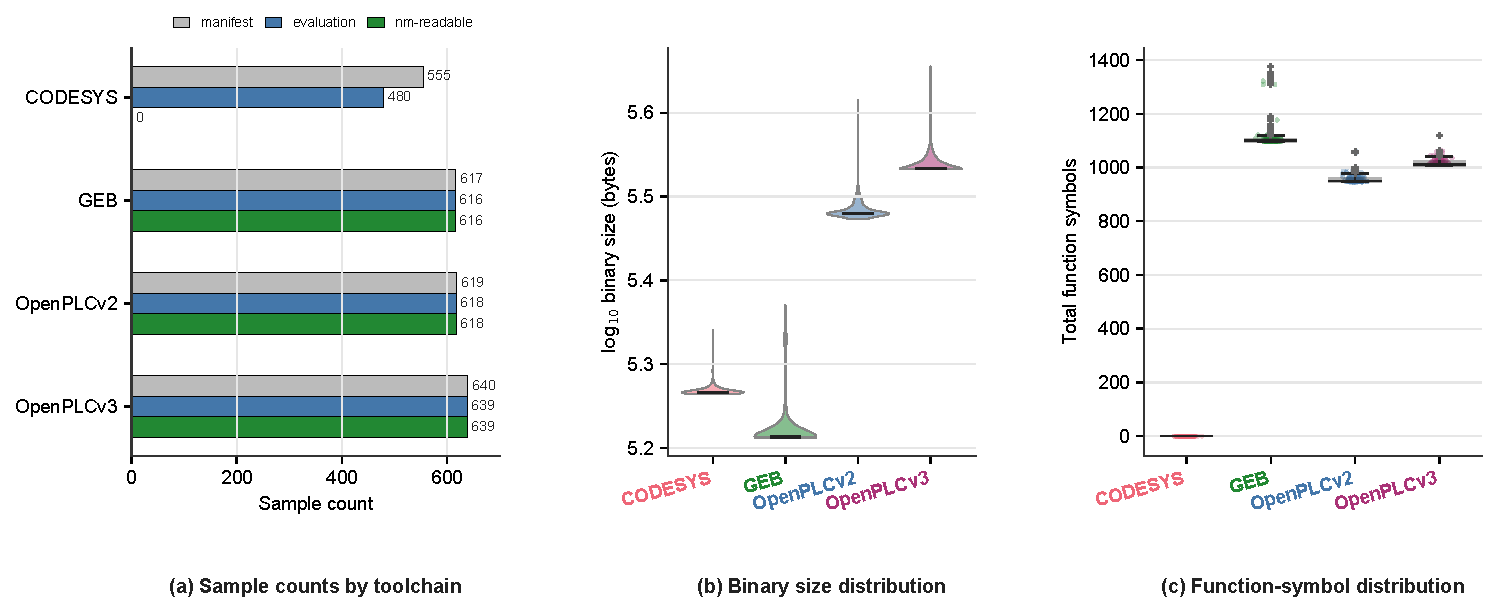
\includegraphics[width=\textwidth]{figs/r1_dataset_observability.pdf}
\Description{Three-panel dataset observability figure. Panel a is a grouped bar chart of manifest, label-available, and nm-readable counts for CODESYS, GEB, OpenPLC v2, and OpenPLC v3. Panel b is a violin plot of log10 binary size in bytes per compiler configuration. Panel c is a box plot with jittered points of emitted function-symbol counts; CODESYS is explicitly marked as nm-unreadable at zero.}
\caption{Tool observability differs by compiler configuration. Panel (a) preserves the original manifest, historical label-available, and historical \texttt{nm}-readable counts; the present card accounting has since been extended to all 2{,}431 rows. Panels (b) and (c) show binary-size and emitted-symbol distributions. A CODESYS value of zero denotes an explained \texttt{nm} tool gap, not a missing sample or absence of control logic.}
\label{fig:dataset}
\end{figure*}

The 78 rows outside the historical classifier subset comprise 75 CODESYS rows and one row from each of GEB, OpenPLC v2, and OpenPLC v3. They carry missing or sentinel function labels, but all have binary paths and split assignments. The v6 rebuild therefore profiles and hashes them, constructs their cards, and includes them in tool-output accounting. It also extends the source oracle to the three non-CODESYS rows. This removes an obsolete label-based selection condition without changing the original 2{,}353 cards: all prior card states and binary hashes match in the regression check.

\subsection{Program-level split protocol}

The split unit is an inferred program name, not a binary row. The \texttt{program\_name} field removes one leading configuration marker (\texttt{codesys\_}, \texttt{geb\_}, \texttt{openplcV2\_}, or \texttt{openplcV3\_}) and the filename extension from \texttt{binary\_name}. This rule produces 714 unique names; all 2{,}431 manifest rows agree with that derivation. Of the 714 names, 458 occur in four configurations, 162 in three, 19 in two, and 75 in one. Each inferred name has one observed \texttt{func\_label}, so no majority resolution is required. Within each label, names are sorted and assigned round-robin to \texttt{fold\_0} through \texttt{fold\_9}. The assignment is deterministic and keeps every observed configuration sharing one inferred name in the same fold.

Let $S$ denote the full manifest sample set, $g(s)$ the inferred name for sample $s$, and $k(g(s))$ its recorded fold. For held-out fold $q$, the test rows are the samples whose inferred name maps to $q$, while the training rows are the remaining samples. The protocol enforces $\{g(s): s \in \mathrm{test}_q\} \cap \{g(s): s \in \mathrm{train}_q\} = \emptyset$, with \texttt{PLCBEAD\_PROGRAM\_LEVEL\_SPLIT.csv} as the authoritative realization. A downstream task may use a subset only when its target is unavailable, as in the source-role oracle; the inclusion reason is recorded separately from the fold assignment.

This inferred-name-disjoint split prevents the same normalized filename from crossing a fold. It does not detect source clones, renamed derivatives, common templates, or algorithm families, and only one deterministic realization is evaluated. Source hashing or token/AST clone grouping is required before this protocol can support a broader unseen-program claim.

\subsection{Scope of nm-based symbol text extraction}

The symbol-extraction stage invokes GNU binutils \texttt{nm}, a symbol-table listing tool, on each input~\cite{gnu_binutils_nm}. It records symbol text already present in the artifact rather than reconstructing absent names. \path{ALL_POPULATION_SAMPLE_FEATURES.csv} contains one status row per manifest sample. The 1{,}876 non-CODESYS rows have status \path{NM_SYMBOLS_RECOVERED}; the 555 CODESYS v3 \texttt{.app} rows emit no symbol text and have status \path{CODESYS_CONTAINER_NOT_RECOVERED}.

These statuses measure tool output, not output correctness. Compiler-generated helpers, truncated tables, or imperfect core/runtime rules could create false-positive or false-negative evidence fields. Section~\ref{sec:source_oracle} introduces source-syntax ground truth for the narrow function-block naming rule, but not for the remaining fields. Stability across optimization levels is also unevaluated. For CODESYS, the observation is limited to the local v3 \texttt{.app} samples and installed tools: no symbol text was emitted for the 555 manifest rows.

\subsection{Leakage logging and protocol controls}

The byte-read protocol is defined separately from the fold assignment. The split file determines which samples belong to each fold, while the leakage audit records whether any feature-generation run reads sample bytes from outside the allowed path or from the wrong split membership. \texttt{V3B\_LEAKAGE\_AUDIT\_PROTOCOL.md} defines the allowlisted PLC-BEAD binary directory, required read mode, required byte-read log columns, and hard-fail conditions. \texttt{V3C\_LEAKAGE\_AUDIT\_SUMMARY.md} summarizes the all-fold audit.

Table~\ref{tab:s3_2} reports the realized split and the scope of the path/membership audit.


\begin{table*}[t]
\centering
\small
\caption{Inferred-name split and path/membership audit protocol.}
\label{tab:s3_2}
\begin{tabularx}{\textwidth}{>{\raggedright\arraybackslash}X>{\raggedright\arraybackslash}X}
\toprule
Protocol dimension & Value \\
\midrule
Split type & Inferred-name-disjoint, label-stratified \\
Folds & 10 \\
Total samples in current card/tool-output population & 2,431 \\
Per-fold approximate current test size & \textasciitilde{}243 \\
Task-specific target handling & Source-role: 1,876 mapped ST rows; historical classifier only: 2,353 label-available rows \\
Leakage allowlist source & \texttt{V3B\_LEAKAGE\_AUDIT\_PROTOCOL.md} \\
Historical leakage log rows (all folds) & 23,530 for the archived 2,353-row classifier surface \\
Full-population v6 identity reads & 2,431; one hash replay per current card \\
Detected path/membership violations & 0 \\
\bottomrule
\end{tabularx}
\end{table*}

The archived all-fold log contains $2{,}353 \times 10=23{,}530$ byte-read rows from the former classifier surface. The v6 rebuild separately replays one binary hash for every current card and confirms all 2{,}431 identities. It does not retroactively relabel the historical all-fold log as a 2{,}431-row experiment. Each logged event stores the sample, fold, train/test membership, resolved path, read mode, byte count, SHA256, allowlist status, and violation status. No path-allowlist or fold-membership violation was detected. This threat model does not cover test-label access, global feature fitting, rule-development feedback, or source-code near duplicates; it therefore does not establish zero statistical leakage.

\subsection{Second-pipeline contract-instantiation set}

The second set is generated independently of the PLC-BEAD \texttt{nm} feature table. It contains 10 hash-profiled x86-64 OpenPLC-derived ELF binaries with 6{,}657 radare2/r2pipe relation rows, eight relation types, and 20 uncertainty records. The relation rows cover function calls, basic-block edges, imports, strings, data references, source/sink hints, patch-affected-function hints, and symbol-to-stripped mappings. The SHA-256 value in every relation and uncertainty record matches the corresponding native-manifest entry.

The adapter uses only observable record properties. Function identifiers populate EC1; static relation rows populate EC3; function-call and basic-block edges populate EC5. Unverified target hints and unavailable declared POU roles remain partial in EC2 and EC4, while the existing static-analysis and label-scope records populate EC6. CVE identifiers and patch roles are retained as provenance but are not used as behavioral labels. This design is a bounded contract-instantiation smoke test across tools and artifact-construction paths. It does not estimate adapter failure on an independently sampled compiler, vendor, or architecture corpus.

\subsection{Protocol summary}

For PLC-BEAD, the manifest defines the sample universe; the split file defines inferred-name membership; the sample-feature file records symbol observability; and the audit protocol records byte-read controls. For the transfer set, the native manifest, relation table, and uncertainty log define the admissible join surface.

A readable-symbol status establishes only that the configured tool emitted names in this environment. A no-symbol status establishes only that this path emitted none. The later evidence cards preserve that observational boundary.


% Source: PAPER1_MANUSCRIPT_S5_SCAA_PLC_FRAMEWORK_DRAFT.md

\section{SCAA-PLC Framework}

\subsection{Framework overview and scope}

SCAA-PLC (Symbol-Consistent Auditable Analysis for PLC binaries) converts binary-analysis observations into structured, inspectable records. In this study, \emph{auditability} is operationalized as traceability from a reported field to its sample, hash, tool output, rule, uncertainty code, and execution log. No human-subject study establishes that analysts interpret the cards more accurately or quickly.

Four terms distinguish the design. The \emph{pipeline} extracts symbol observations and constructs graph/card records. The \emph{framework} combines that pipeline with the evidence schema, uncertainty taxonomy, and audit controls. The \emph{protocol} specifies program splitting and admissible byte reads. The resulting \emph{reporting layer} sits between raw tool output and downstream interpretation.

Table~\ref{tab:scope} fixes the interpretation boundary once for the remainder of the paper. Here, ``evidence'' means a reproducible observation produced by the configured pipeline, such as an \texttt{nm}-emitted name, a rule-table match, or a recorded uncertainty event. Figure~\ref{fig:framework} shows how the manifest, split, symbol observations, graph records, evidence cards, and audit logs connect.

\begin{table*}[t]
\centering
\small
\caption{Evaluated scope and evidence required for broader claims.}
\label{tab:scope}
\begin{tabularx}{\textwidth}{>{\raggedright\arraybackslash}X>{\raggedright\arraybackslash}X>{\raggedright\arraybackslash}X}
\toprule
Evaluated & Not evaluated & Evidence required to extend scope \\
\midrule
PLC-BEAD sample accounting; \texttt{nm}-emitted symbols; source-syntax agreement and ungated transfer for one GEB pattern; two/three/six-slot information retention; native OpenPLC/radare2 record adaptation; path/membership audit & Runtime state machines; validated function boundaries; vulnerability detection; physical-process behavior; analyst decision utility; universal CODESYS support; cross-vendor generalization & Format-aware recovery oracle; independent vendor corpora; clone-aware repeated splits; controlled analyst study; task-level or behavioral validation \\
\bottomrule
\end{tabularx}
\end{table*}

\begin{figure*}[t]
\centering
\includegraphics[width=\textwidth]{figs/fig1_scaa_plc_framework_revision.pdf}
\Description{Four-lane SCAA-PLC evidence construction framework schematic. The lanes show PLC-BEAD accounting and read discipline, observable evidence with an nm-readable branch and a CODESYS no-symbol branch, a reporting layer containing EC1 through EC6 fields, and outputs for source-oracle validation, uncertainty, and execution auditing.}
\caption{SCAA-PLC preserves a trace from each raw observation to an evidence field, uncertainty code, and execution audit record.}
\label{fig:framework}
\end{figure*}

\subsection{Design requirements and contract invariants}

The schema was derived from five reporting requirements rather than from an assumption that six fields are independent constructs. DR1 preserves sample identity through a content hash. DR2 keeps each observation traceable to its tool output or source rule. DR3 distinguishes an unsupported observation from a negative finding. DR4 requires a typed uncertainty event for every weak evidence field. DR5 keeps run and join provenance machine-checkable. These requirements connect empirical-study reporting~\cite{kitchenham_reporting2008,revoredo_reporting2021}, metadata-driven experimentation~\cite{santana_metadata2026}, computational provenance~\cite{freire_provenance2008}, and explicit binary-analysis uncertainty~\cite{euba_sandia2021} to the PLC-binary setting.

The initial slot and U-code vocabulary was exercised against three observed failure families: a CODESYS container/tool mismatch, ambiguous declared state-role evidence, and cross-pipeline relation/label-scope uncertainty. All six EC slots are instantiated in the primary population. Five uncertainty codes (U01, U02, U11, U13, and U09b) occur in the current construction; non-applicability is stored separately, and the remaining defined codes are not observed in this population. This does not demonstrate taxonomy saturation. No independent coder-agreement or expert content-validation study has yet established necessity or completeness. EC1--EC6 and U01--U14 are consequently treated as chosen provenance categories with measured coverage, not as a universal taxonomy.

Five positive invariants make the implemented guarantee testable: (I1) every card hash replays against its binary; (I2) every weak EC1--EC5 slot has an uncertainty event; (I3) configured-tool gaps remain partial rather than negative; (I4) every mapped source hash replays against its source bytes; and (I5) every second-pipeline relation or uncertainty hash joins its manifest entry. Section~5 reports the checked units and failures for each invariant.

\subsection{Evidence-card structure}

The evidence card connects per-sample tool observations to evaluation. Its primary output is the raw vector $(f_1,\ldots,f_6)$ together with supporting row identifiers and uncertainty codes. Each slot states whether a defined evidence type has direct support, explained partial support, or unexplained absence. The six slots are provenance categories rather than assumed independent statistical constructs. Table~\ref{tab:s5_1} gives each slot, fill rule, and uncertainty handoff.


\begin{table*}[t]
\centering
\small
\caption{Evidence-card fields and fill decisions.}
\label{tab:s5_1}
\begin{tabularx}{\textwidth}{>{\raggedright\arraybackslash}p{0.08\textwidth}>{\raggedright\arraybackslash}p{0.22\textwidth}>{\raggedright\arraybackslash}X>{\raggedright\arraybackslash}p{0.18\textwidth}}
\toprule
Slot & Purpose & Fill rule & Uncertainty handoff \\
\midrule
EC1 & Function-candidate availability & \texttt{1} if a candidate exists; \texttt{0.5} if a format/tool uncertainty explains absence; \texttt{0} if absent without explanation & U01/U02/U04 \\
EC2 & Core/control-logic candidate status & \texttt{1} if fixed core-rule provenance supports a core/control hint; \texttt{0.5} if assignment is weak; \texttt{0} if absent without explanation & U05/U13 \\
EC3 & Static-fact availability & \texttt{1} if static fact rows exist; \texttt{0.5} if unavailable with tool or relation uncertainty; \texttt{0} otherwise & U06/U07/U08/U11 \\
EC4 & Declared state-role evidence & \texttt{1} if declared state-role naming is supported; \texttt{0.5} if attempted but weak; \texttt{0} if absent without explanation & U08/U09a/U09b/U13 \\
EC5 & Relation-graph availability & \texttt{1} if non-uncertainty evidence edges exist; \texttt{0.5} if only uncertainty edges explain the gap; \texttt{0} otherwise & U02/U06/U07/U08/U12 \\
EC6 & Uncertainty-log coverage & \texttt{1} if every weak/missing field has a U-code event; \texttt{0.5} if some do; \texttt{0} otherwise & U01..U14 \\
\bottomrule
\end{tabularx}
\end{table*}

EC2 uses the fixed core/runtime table described in Section~\ref{sec:state_adapter}; EC6 checks whether every weak field has an associated U-code. For a sample $s$, each fill $f_i(s)$ is 0, 0.5, or 1, denoting unexplained absence, explained partial support, and direct support. The six-slot vector and its trace rows are the reported method outputs. No weighted aggregate is used by the revised method.

\paragraph{Worked example.} Three observed cards illustrate the fill semantics. The GEB sample \texttt{geb\_ARRAY\_HAV} has direct support in EC1--EC6. Its EC4 support includes an SA-001 match on the in-binary \texttt{dt\_FB\_} function-block naming pattern; its source file separately declares a \texttt{FUNCTION\_BLOCK}. The GEB sample \texttt{geb\_AIN} has filled EC1, EC2, EC3, EC5, and EC6, but its source declares a \texttt{FUNCTION} and EC4 remains partial with U09b. In contrast, \texttt{codesys\_\_ARRAY\_ABS} produces no \texttt{nm} output: EC1--EC5 are partial with recorded uncertainty, while EC6 records that coverage. The vectors distinguish direct source agreement, explained partial support, and a configured tool gap without converting missing output into a semantic finding.

\paragraph{EC-field co-fill structure.} EC1, EC2, EC3, and EC5 have zero row-level status mismatches on all 2{,}431 PLC-BEAD cards. EC4 varies with state-adapter output, while EC6 is filled for every row. The six slots therefore encode three empirical channels on PLC-BEAD. They remain separate trace categories because the second-pipeline adapter produces a different slot pattern, including direct function/graph evidence with partial claim support.

The card is thus a reporting contract rather than a six-dimensional quality scale. The evaluation directly compares reduced representations; whether any representation improves human decisions remains an open empirical question.

\subsection{Uncertainty taxonomy}

The uncertainty taxonomy records why evidence is weak, missing, or tool-dependent. A single missing-data flag would collapse format boundaries, architecture ambiguity, relation partiality, state-role ambiguity, metadata gaps, and tool failure into one bucket. SCAA-PLC instead groups U-codes by evidence failure mode so that later tables can report what type of limitation occurred.

Table~\ref{tab:s5_2} groups the U-codes by the evidence boundary that each event records.


\begin{table*}[t]
\centering
\small
\caption{Uncertainty-code families.}
\label{tab:s5_2}
\begin{tabularx}{\textwidth}{>{\raggedright\arraybackslash}X>{\raggedright\arraybackslash}X>{\raggedright\arraybackslash}X}
\toprule
Family & Codes & Role in the framework \\
\midrule
Format/container/architecture & U01, U02, U03 & Input format, container parsing, or architecture confirmation is unavailable. \\
Function and core/runtime evidence & U04, U05 & Function-boundary candidate or core/runtime assignment is partial or unstable. \\
Static relation and data evidence & U06, U07, U08 & Control-flow graph (CFG), call, or data-flow evidence is partial or tool-dependent. \\
State-role evidence & U09 (deprecated umbrella; replaced by U09a and U09b), U09a, U09b & U09a means the state adapter was not attempted; U09b means it was attempted but only weak, generic, or ambiguous evidence was available. \\
Metadata/tool/human-review/not-applicable & U10, U11, U12, U13, U14 & Metadata gaps, tool failure, tool disagreement, human-review need, or non-applicability. \\
\bottomrule
\end{tabularx}
\end{table*}

Uncertainty coverage records where the evidence path stops and which later review or tool step could narrow it. Supplementary Fig.~S2 reports per-configuration and overall U-code frequencies. CODESYS rows resolve almost entirely to U01; non-CODESYS rows distribute their primary codes across U09b (state adapter attempted but weak) and U14 (stored as \texttt{NOT\_APPLICABLE}).

The taxonomy is ordered to preserve reviewer-auditable provenance. Format and container issues appear before graph-level issues because later graph records cannot be interpreted if the input representation is not stable. State-role uncertainty is split from relation uncertainty because a sample can have call or control-flow evidence without supporting declared state-role evidence. Tool failure and tool disagreement are separated because a missing output from one tool has a different evidentiary meaning from conflicting outputs across tools. Human-review-required marks cases where automated evidence is insufficient for a final interpretation. Defined but unobserved codes remain in the specification to make their intended handling explicit; they are not counted as empirical coverage.

\subsection{State-adapter rule families}
\label{sec:state_adapter}

The state-adapter (SA) layer applies fixed naming rules to emitted symbol text or PLC-BEAD metadata. SA-001--SA-004 are symbol-derived; SA-005--SA-020 are metadata-derived controls.

SA-001 matches the \texttt{dt\_FB\_} pattern observed in GEB symbol text; the fixed rule interprets that pattern as declared function-block naming and directly fills EC4. It is an empirical GEB convention in PLC-BEAD, not an IEC 61131-3 binary naming rule. SA-002--SA-004 retain program or cyclic-execution context without independently filling EC4. The metadata rules match timer, counter, input, output, memory, and latch terms in \texttt{program\_name} or \texttt{binary\_name}.

Table~\ref{tab:s5_3} summarizes the symbol-derived rule families used in the reported evaluation.

\begin{table*}[t]
\centering
\small
\caption{State-adapter rule families used for declared PLC naming evidence.}
\label{tab:s5_3}
\begin{tabularx}{\textwidth}{>{\raggedright\arraybackslash}X>{\raggedright\arraybackslash}X>{\raggedright\arraybackslash}X>{\raggedright\arraybackslash}X}
\toprule
Rules & Scope & Match field & Recorded contribution \\
\midrule
SA-001 & GEB & \texttt{core\_symbol\_text}: \texttt{dt\_FB\_} & Direct declared function-block evidence; fills EC4 \\
SA-002--SA-004 & GEB/OpenPLC v2/v3 & \texttt{core\_symbol\_text}: program/cyclic patterns & Context records only; do not independently fill EC4 \\
\bottomrule
\end{tabularx}
\end{table*}

Full regular expressions remain in \texttt{V3\_STATE\_ADAPTER\_RULES.csv}. The evaluation separates the symbol and metadata families without changing their definitions.

\subsection{Construction procedure and implementation controls}

The implementation accepts either the PLC-BEAD manifest path or an explicitly marked synthetic-fixture path; other inputs hard-fail. Dataset runs also enforce the split membership and byte-read allowlist. Algorithm~\ref{alg:evidence_card} states the concrete record-construction order.

\begin{algorithm}[tbp]
\caption{Evidence-card construction}
\label{alg:evidence_card}
\begin{algorithmic}[1]
\Require sample $s$, manifest/split, symbol record, fixed rule tables
\State Verify sample membership, path allowlist, and input mode; otherwise hard-fail
\State Read the binary once, record byte count and SHA256, and log fold membership
\State Set EC1 from \texttt{nm}-emitted function candidates
\State Set EC2 from the 17-row core/runtime rule table
\State Set EC3 and EC5 from emitted fact rows and non-uncertainty graph edges
\State Set EC4 from fixed SA rules; only SA-001 gives direct symbol-derived support
\State For a missing direct predicate, assign 0.5 only when a qualifying U-code exists
\State Set EC6 from coverage of all weak/missing fields by U-code events
\State Select \texttt{primary\_missing\_reason} by severity, field order, then U-code
\State Emit graph, card, uncertainty, and byte-read records
\end{algorithmic}
\end{algorithm}

The manifest, split, feature, graph, card, uncertainty, and byte-read files together form the reproducibility contract evaluated next.


% Source: PAPER1_MANUSCRIPT_S6_EVALUATION_DRAFT.md

\section{Evaluation}

\subsection{Evaluation scope}

Under Table~\ref{tab:scope}, the evaluation addresses the three research questions through (i) a source-syntax test that separates a scoped production rule from an ungated transfer probe, (ii) a fold-wise comparison of two-, three-, and six-slot representations, and (iii) a bounded adapter test over a separately generated radare2 evidence set. Full-population card construction, five contract invariants, path/membership auditing, and synthetic regression provide implementation controls. Historical one-fold classifiers and EC4 spread diagnostics are excluded from the submission supplement and retained only in the artifact's non-contributory history directory.

\subsection{Evaluation artifacts and source traceability}

The evaluation uses the hash-addressed card, uncertainty, source-oracle, contract-invariant, and JSS validation packages. The v6 package adds 2{,}431-row features and cards, a 1{,}876-row source oracle, RQ-specific population flow, fold-wise schema predictions, trace cases, schema coverage, and invariant results. The GitHub-ready artifact release candidate packages the derived inputs selected for reviewer verification under package-relative paths, compresses the 195-MiB feature table, records file checksums, and provides a one-command validator plus a clean-room log. Raw PLC-BEAD binaries and sources are not redistributed because the examined upstream snapshot contains no explicit license file; a verifier checks a separately acquired snapshot against the card and source hashes. A reviewer URL, archival DOI, and author-selected code/data licenses remain human submission actions, so the package is not yet described as publicly available.

\subsection{Evaluation setup}

The source-syntax analysis uses exact confusion counts because it evaluates every row with a reliable Structured Text mapping in the local snapshot rather than sampling from a declared population. Card/tool-output accounting uses all 2{,}431 manifest rows. The schema comparison uses the frozen ten-fold inferred-name assignment. For each fold, a transparent signature-majority decoder learns the majority target value for each observed card signature from the other nine folds and predicts the held-out fold. Every included sample is predicted once. The experiment measures information retained by the representation; it is neither a learned production model nor a test of analyst utility. The second-pipeline adapter uses only hashes, relation records, function identifiers, and uncertainty rows already emitted by that pipeline.

\subsection{Source-syntax oracle validity test}
\label{sec:source_oracle}

The separately extracted oracle removes Structured Text comments and extracts line-anchored \texttt{FUNCTION\_BLOCK}, \texttt{FUNCTION}, and \texttt{PROGRAM} declarations from the same PLC-BEAD snapshot. A binary row is mapped to source files with the same normalized program stem within its compiler configuration. Multiple matching files are accepted only if they agree on explicit \texttt{FUNCTION\_BLOCK} presence. This is a syntactic POU-role oracle, not runtime-state or source-to-binary semantic ground truth.

Two distinct tests prevent a scope gate from predetermining the transfer result. The production SA-001 rule requires GEB and \texttt{dt\_FB\_}; OpenPLC is therefore \texttt{OUT\_OF\_SCOPE}, not negative. The ungated probe removes only the GEB condition and applies the unchanged lexical predicate to GEB, OpenPLC v2, and OpenPLC v3. Table~\ref{tab:source_oracle} reports exact row counts. On 617 GEB rows, the production predicate and the identical ungated predicate agree with 353 source-positive and 264 source-negative rows. The ungated probe emits no positives on either OpenPLC configuration despite 735 source-positive rows.

\begin{table*}[t]
\centering
\small
\caption{The production rule is GEB-scoped; a separate ungated lexical probe has zero recall on the evaluated OpenPLC configurations.}
\label{tab:source_oracle}
\begin{tabularx}{\textwidth}{>{\raggedright\arraybackslash}X>{\raggedright\arraybackslash}p{0.12\textwidth}rrrrrrrr}
\toprule
Configuration & Production scope & $n$ & Source FB & Probe + & TP & FP & FN & TN & Recall \\
\midrule
GEB & In scope & 617 & 353 & 353 & 353 & 0 & 0 & 264 & 1.000 \\
OpenPLC v2 & Out of scope & 619 & 359 & 0 & 0 & 0 & 359 & 260 & 0.000 \\
OpenPLC v3 & Out of scope & 640 & 376 & 0 & 0 & 0 & 376 & 264 & 0.000 \\
\bottomrule
\end{tabularx}
\end{table*}

The OpenPLC rows are out of scope for the production SA-001 rule. The 735 OpenPLC false negatives belong only to the ungated probe. They show that \texttt{dt\_FB\_} is an evaluated GEB naming convention rather than a compiler-independent function-block marker. RQ1 is therefore a bounded, post-hoc validity case: the scoped rule agrees with the same-snapshot source oracle in GEB, whereas its lexical predicate does not transfer to either evaluated OpenPLC compiler. The rule-development and confirmation data are not independent, so the zero-error GEB count is not interpreted as prospective accuracy.

\subsection{End-to-end trace cases}

Table~\ref{tab:trace_cases} carries the running example into the evaluation. Each row starts from an observed tool record, identifies the governing rule or provenance boundary, and ends with the strongest allowed conclusion. The machine-readable table also stores the binary/source hashes and full row identifiers.

\begin{table*}[t]
\centering
\scriptsize
\caption{Three trace chains distinguish direct source agreement, source-negative contrast, and an explained tool gap.}
\label{tab:trace_cases}
\begin{tabularx}{\textwidth}{>{\raggedright\arraybackslash}p{0.13\textwidth}>{\raggedright\arraybackslash}p{0.22\textwidth}>{\raggedright\arraybackslash}p{0.18\textwidth}>{\raggedright\arraybackslash}p{0.18\textwidth}>{\raggedright\arraybackslash}X}
\toprule
Sample & Raw observation / provenance & EC1--EC6 & Oracle / U-code & Allowed conclusion \\
\midrule
\texttt{geb\_ARRAY\_HAV} & 1,104 \texttt{nm} function symbols; GEB-scoped \texttt{dt\_FB\_}; mapped \texttt{ARRAY\_HAV.ST} & filled / filled / filled / filled / filled / filled & Source \texttt{FUNCTION\_BLOCK}; no U-code & Lexical rule and source syntax agree for this row; runtime semantics do not follow. \\
\texttt{geb\_AIN} & 1,100 symbols; \texttt{dt\_FN\_AIN}; mapped \texttt{AIN.ST} & filled / filled / filled / partial / filled / filled & Source \texttt{FUNCTION}; U09b & Source-negative contrast supports the GEB naming boundary, not compiler independence. \\
\texttt{codesys\_\_ARRAY\_ABS} & CODESYS \texttt{.app}; configured \texttt{nm} path emits zero symbols & partial / partial / partial / partial / partial / filled & No reliable ST oracle; U01/U02/U11/U13 & The tool path is unsupported for this row; absence of PLC logic is not inferred. \\
\bottomrule
\end{tabularx}
\end{table*}

The aggregate statement ``all PLC-BEAD binaries expose \texttt{nm}-readable functions'' is rejected by the third trace, while ``unsupported output proves absence of control logic'' is rejected by its partial fields and uncertainty closure. This demonstrates claim tracing by construction. Whether reviewers reach these decisions more accurately or quickly with the card remains an unexecuted human-study question.

\subsection{Schema economy}

The comparison defines three representations. \texttt{S2} contains tool-output observability and uncertainty coverage; \texttt{S3} contains the three empirical PLC-BEAD channels (observability, EC4 state-role evidence, and uncertainty); and \texttt{S6} retains all six typed trace slots. Two binary targets are used: whether the configured tool emitted function candidates for each of all 2{,}431 rows, and whether a mapped source file explicitly declares a function block for the 1{,}876 source-mapped non-CODESYS rows. The latter is a source-syntax information-retention task, not a semantic-recovery task.

Table~\ref{tab:schema_economy} reports the fold-wise decoder results. All three schemas exactly retain the tool-output boundary. For source function-block presence, \texttt{S3} and \texttt{S6} have identical confusion counts and metrics, while \texttt{S2} predicts only the fold-majority class. The collision audit also finds zero status mismatches among EC1, EC2, EC3, and EC5 on all 2{,}431 cards. Thus, the six-slot representation adds no measured discrimination over three empirical channels for these tasks, although it retains distinct provenance categories for record inspection and bounded cross-pipeline instantiation.

\begin{table*}[t]
\centering
\scriptsize
\caption{Fold-wise information retention by reduced and full evidence-card representations.}
\label{tab:schema_economy}
\begin{tabularx}{\textwidth}{>{\raggedright\arraybackslash}Xlrrrrrr}
\toprule
Target & Schema & $n$ & Acc. & Bal. acc. & Macro F1 & Signatures & Ambig. rows \\
\midrule
Tool output & S2 & 2,431 & 1.000 & 1.000 & 1.000 & 2 & 0 \\
Tool output & S3 & 2,431 & 1.000 & 1.000 & 1.000 & 3 & 0 \\
Tool output & S6 & 2,431 & 1.000 & 1.000 & 1.000 & 3 & 0 \\
Source function block & S2 & 1,876 & 0.580 & 0.500 & 0.367 & 1 & 1,876 \\
Source function block & S3 & 1,876 & 0.648 & 0.692 & 0.638 & 2 & 1,876 \\
Source function block & S6 & 1,876 & 0.648 & 0.692 & 0.638 & 2 & 1,876 \\
\bottomrule
\end{tabularx}
\end{table*}

Every source-task signature is ambiguous in the full corpus because the evidence channels do not uniquely identify source POU role. The reported majority decoder is therefore a controlled probe of retained information, not a useful source-role classifier. RQ2 supports three channels as the empirically sufficient statistical representation on PLC-BEAD; six slots remain the trace-preserving reporting form. Human-facing usefulness of that extra structure remains untested.

\subsection{Contract-invariant validation}

Table~\ref{tab:invariants} reports the positive guarantees defined in Section~4. The checks replay raw hashes or row-level joins; none is inferred from a reported aggregate. All five invariants pass with zero failures.

\begin{table*}[t]
\centering
\small
\caption{All evaluated record-contract invariants pass; checked units differ by invariant and are not accuracy denominators.}
\label{tab:invariants}
\begin{tabularx}{\textwidth}{>{\raggedright\arraybackslash}p{0.18\textwidth}r r>{\raggedright\arraybackslash}X}
\toprule
Invariant & Checked units & Failures & Checked property \\
\midrule
I1 identity hash & 2,431 & 0 & Card SHA-256 replays against each primary binary. \\
I2 uncertainty closure & 4,176 & 0 & Every weak EC1--EC5 slot has a typed uncertainty row. \\
I3 unsupported-not-negative & 555 & 0 & CODESYS tool gaps remain partial rather than unexplained missing/negative. \\
I4 source trace & 1,876 & 0 & Mapped source SHA-256 replays against source bytes. \\
I5 cross-pipeline hash join & 6,677 & 0 & Relation and uncertainty hashes join the native manifest. \\
\bottomrule
\end{tabularx}
\end{table*}

The guarantees are deliberately record-level. I2 shows that weak fields are explained, not that the explanation is correct; I3 prevents one class of overinterpretation, not every possible analyst error; and I5 establishes referential integrity rather than relation correctness.

\subsection{Bounded second-pipeline contract instantiation}

The second test instantiates one evidence card for each of 10 OpenPLC-derived ELF binaries from a separately implemented radare2/r2pipe construction path. Table~\ref{tab:cross_pipeline} summarizes the join checks. All relation and uncertainty rows join to the native manifest by sample identifier and SHA256. All cards contain function identifiers and graph relations, and each contains uncertainty from both static-analysis and label-scope stages.

\begin{table*}[t]
\centering
\small
\caption{Record-contract instantiation over the second native OpenPLC/radare2 pipeline.}
\label{tab:cross_pipeline}
\begin{tabularx}{\textwidth}{>{\raggedright\arraybackslash}Xr>{\raggedright\arraybackslash}X}
\toprule
Record check & Count & Result \\
\midrule
Hash-profiled native binaries / adapted cards & 10 & All manifest SHA256 joins match \\
Static relation records & 6,657 & Eight relation types; all sample/hash joins match \\
Uncertainty records & 20 & Two recorded uncertainty stages per card \\
Cards with function and graph records & 10 & Function IDs and graph relations present for every card \\
\bottomrule
\end{tabularx}
\end{table*}

The different slot pattern is material: function and graph observations directly support EC1, EC3, and EC5, while the absence of verified target semantics and declared POU roles leaves EC2 and EC4 partial; EC6 records those boundaries. RQ3 is therefore supported only as a bounded contract instantiation. The adapter assigns states using explicit mapping rules, and the 10 binaries are all OpenPLC-derived GCC/x86-64 artifacts. This smoke test does not estimate mapping failures on another compiler, vendor, architecture, or independently implemented adapter.

\subsection{Leakage and regression checks}

These checks validate implementation behavior separately from the three research questions. CODESYS rows have partial EC1--EC5 fields because the evaluated \texttt{nm} path emitted no symbols; EC6 records the associated uncertainty coverage.

The historical byte-read audit flags an event when its resolved path is outside the allowlist or its recorded inferred-name fold disagrees with run membership. None of the 23{,}530 events is flagged. The row count is the Cartesian check of the archived 2{,}353-row classifier surface across ten runs, not 23{,}530 distinct binaries. The v6 current-population rebuild adds 2{,}431 direct hash reads and finds no identity mismatch. As defined in Section~3.4, these results cover logged path, membership, and identity properties only.

Regression uses four hand-crafted fixtures: complete OpenPLC evidence, a CODESYS-like format gap, partial state evidence, and unexplained missing fields. Those fixtures generate six reference output tables whose normalized SHA256 values remain unchanged after the rule-priority and mode-guard revision. They exercise specified branches; they do not validate behavior on additional real binaries. Historical classifier and ablation diagnostics are preserved under \path{history/} in the artifact but do not contribute to the current RQs.

Together these controls expose which bytes were read, which rules generated each table, and whether a maintenance change altered the synthetic reference behavior.

\subsection{Evaluation summary}

SCAA-PLC constructs traceable records for all 2{,}431 PLC-BEAD binaries. The source oracle establishes a bounded GEB naming case and exposes complete lexical-transfer failure on the evaluated OpenPLC compilers. Three empirical channels retain the same evaluated information as six typed slots, while two fields lose source-role information. Five contract invariants pass with zero failures, and the second radare2 path instantiates the contract without a hash-join failure. These results establish full-population accounting, trace closure, schema economy, and bounded implementation feasibility. They do not establish human utility, taxonomy completeness, semantic accuracy, or vulnerability-detection effectiveness.


% Source: PAPER1_MANUSCRIPT_S7_DISCUSSION_DRAFT.md

\section{Discussion, Limitations \& Related Contrast}

\subsection{CODESYS boundary under the evaluated tools}

The most important configured boundary is the local PLC-BEAD CODESYS v3 \texttt{.app} subset. All 555 manifest rows provide no \texttt{nm}-readable symbols under the configured path and remain in current card-level accounting; the former 480/2{,}353 count describes only the historical label-available subset. Keeping all 555 prevents a function-label gate from obscuring the dataset--tool interface.

Table~\ref{tab:s7_1} distinguishes this configured-tool result from format-specific CODESYS capabilities reported elsewhere.


\begin{table*}[t]
\centering
\small
\caption{The evaluated generic-tool path emits no functions for the sampled CODESYS v3 containers; format-specific prior work prevents a universal opacity claim.}
\label{tab:s7_1}
\begin{tabularx}{\textwidth}{>{\raggedright\arraybackslash}X>{\raggedright\arraybackslash}X>{\raggedright\arraybackslash}X>{\raggedright\arraybackslash}X}
\toprule
Aspect & Observation & Scope / interpretation & Source artifact \\
\midrule
Current CODESYS card/tool-output population & 555/2431 manifest rows; all are explained tool gaps & Installed public-tool and local \texttt{.app} scope & \path{ALL_POPULATION_SAMPLE_FEATURES.csv}; \path{ALL_POPULATION_EVIDENCE_CARDS.csv} \\
Local PLC-BEAD CODESYS manifest subset & 555/2431 manifest rows & PLC-BEAD inventory scope only; not a claim about all CODESYS artifacts. & \path{PLCBEAD_MANIFEST.csv}; \path{CODESYS_APP_FORMAT_INVESTIGATION.md} \\
Local public-tool trial & Five sampled \texttt{.app} files identified as \texttt{data}; radare2 default loader reported \texttt{havecode false} and function count 0 & Bounded five-file probe & \path{CODESYS_TOOL_TRIAL_LOG.md}; \path{CODESYS_TOOL_TRIAL_RESULTS.csv} \\
Recorded tool environment & GNU nm 2.38; file 5.41; radare2 6.1.9 with recorded library path; local binwalk 2.3.3; project-venv unblob 26.6.4 & Versioned environment for this study; not a universal tool capability assessment & \path{CODESYS_TOOL_ENV_STATE.md} \\
ICSREF runtime gap for local PLC-BEAD CODESYS use & Python 2.7 required; \texttt{python2.7} and \texttt{python2} not found locally & Compatibility assessment only; not a full configured ICSREF run. & \path{CODESYS_ICSREF_COMPATIBILITY_REPORT.md} \\
ICSREF format gap for local PLC-BEAD CODESYS use & ICSREF CLI expects \texttt{.PRG}; local PLC-BEAD samples are v3-style \texttt{.app} files & Local \texttt{.app} scope; no claim about ICSREF on intended v2 \texttt{.PRG} inputs. & \path{CODESYS_ICSREF_COMPATIBILITY_REPORT.md} \\
ICSREF parser assumptions for local PLC-BEAD CODESYS use & v2 PRG header offsets at \texttt{0x20}, \texttt{0x2C}, and \texttt{0x44}; ARM prologue/epilogue heuristics & Header assumptions are not validated for local \texttt{.app} samples; no compatibility bridge attempted here. & \path{CODESYS_ICSREF_COMPATIBILITY_REPORT.md} \\
\bottomrule
\end{tabularx}
\end{table*}

The ICSREF rows explain why a framework for CODESYS v2 \texttt{.PRG} input is not directly applicable to the local v3 \texttt{.app} files.

\paragraph{Observed boundaries.} In the five-file probe recorded by \texttt{CODESYS\_TOOL\_TRIAL\_RESULTS.csv}, \texttt{file(1)} reports generic \texttt{data} rather than an Executable and Linkable Format (ELF) or Portable Executable (PE) file, so \texttt{nm} emits no symbol table. The radare2 default loader reports \texttt{havecode false} and zero functions. Neither \texttt{binwalk} nor \texttt{unblob} matches a supported extraction signature. These observations support the U01 format/container handling applied to the 555 current CODESYS cards. Because only five containers were probed with those additional tools, this is a bounded tool trial rather than proof that all CODESYS formats are intrinsically opaque.

\subsection{Measurement validity and framework complexity}

The full boundaries are defined in Table~\ref{tab:scope}. Within that scope, four validity gaps matter. First, the source oracle validates only explicit \texttt{FUNCTION\_BLOCK} syntax for one post-hoc lexical predicate; EC1--EC3 and EC5 still inherit possible errors from configured-tool output and fixed rules. Second, the schema tasks measure information retention under a transparent signature decoder, not whether an analyst reaches a better or faster decision. Third, ``inspectable'' means artifact-level traceability in this study; the artifact includes a counterbalanced reviewer-task protocol, but no human result is reported. Fourth, slot and U-code coverage does not replace independent coder agreement, expert content validation, or saturation testing.

EC1, EC2, EC3, and EC5 co-fill perfectly on PLC-BEAD, leaving three effective statistical channels. The explicit schema comparison shows that the three-channel and six-slot representations are indistinguishable on the two evaluated information-retention tasks, whereas the two-field summary loses source-role information. The six-slot layout is therefore justified here as a provenance decomposition, not as six independent predictive dimensions. The five invariants make that decomposition falsifiable at the record level. A controlled reviewer study is still required to determine whether those categories improve decision quality enough to justify their presentation cost.

\subsection{Related contrast}

Ta'veren recovers binary-level state machines, PLC-BinX analyzes function boundaries and code regions, and ICSREF targets CODESYS v2 \texttt{.PRG} inputs. CLEVER and CLADF evaluate stronger decompilation or run-time integrity tasks. SCAA-PLC records the provenance and limits of a lighter public-tool path. The radare2 adapter shows that relation-rich outputs can populate the same reporting contract, but no format-aware CODESYS integration or semantic-equivalence test is included.

For empirical software evaluation and review, this separates observable PLC-binary support from format-induced tool gaps before downstream conclusions are drawn.

\subsection{Limits on generalization}

The source-rule and schema evaluations cover one public corpus and one deterministic inferred-name split. The second pipeline changes the extraction tool and record shape, but its binaries are also OpenPLC-derived x86-64 artifacts; it is not an independent vendor or architecture population. Broader generalization requires source-clone grouping, repeated split realizations, independently sourced PLC corpora, optimization/compiler perturbations, and format-aware CODESYS processing. The study also contains no PLC execution, plant model, physical-process outcome, or completed analyst decision task. Consequently, RQ3 establishes only bounded second-pipeline contract instantiation, not record portability across PLC ecosystems.

\subsection{Ethics and broader impact}

The study uses a public benchmark and emits no exploit, vulnerability verdict, vendor identification, or deployment recommendation. Explicitly retaining unsupported samples and tool assumptions supports responsible reuse because downstream readers can distinguish missing evidence from a negative semantic finding.


% Source: PAPER1_MANUSCRIPT_S8_CONCLUSION_DRAFT.md

\section{Conclusion}

SCAA-PLC converts PLC binary-analysis observations into per-sample records that retain rule provenance, typed uncertainty, hashes, and execution controls. The current build covers all 2{,}431 manifest binaries and 1{,}876 source-mapped rows. A separately extracted source oracle provides a bounded GEB naming case, while an ungated probe shows that the same lexical predicate does not transfer to the evaluated OpenPLC compilers. Three empirical channels retain the same evaluated task information as six trace slots, and a second radare2 path provides a bounded contract instantiation for 10 binaries and 6{,}657 relations. Five positive invariants pass with zero failures, including identity, uncertainty closure, source trace, unsupported-sample handling, and cross-pipeline joins. The methodological implication is that observations, support boundaries, uncertainty, and execution provenance should remain distinct from aggregate outcomes. Independent corpora, independent schema validation, format-aware CODESYS analysis, and controlled analyst tasks are required before broader portability, effectiveness, or utility claims are justified.


\begin{acks}

This work was supported by the Liaoning Provincial Science and Technology Major Projects under Grant No.~2026JH1/11700024; the Liaoning Provincial Applied Basic Research Programs under Grant Nos.~2025JH2/101300012 and 2026JH2/101300068; the 2026 Central Government-Guided Local Science and Technology Development Program of Liaoning Province for Regional Innovation System Development under Grant No.~[2026]48(4); and the 2026 Liaoning Provincial International Industrial Technology Research and Development Program under Grant No.~[2026]60(3).

\end{acks}

\section*{Data Availability Statement}

The PLC-BEAD corpus is obtainable from \url{https://github.com/AICPS/PLCBEAD_PLCEmbed} (examined commit \texttt{b9593436eb36d1c7847870207692b6b2eb7747c3}). Because that snapshot contains no explicit license file, the release candidate does not redistribute its raw binaries or sources. It provides a hash verifier for a separately acquired copy. The package includes author-generated manifests, all-population cards, source-oracle outputs, schema predictions, contract-invariant results, trace cases, cross-pipeline derived tables, fixtures, checksums, environment notes, and a one-command clean-room validator. A public reviewer URL, archival DOI, release tag, and author-approved code/data licenses remain unassigned and must be supplied before submission; until then, the package is an internal release candidate rather than a public artifact. No proprietary firmware, vendor artifact, or human-subject result is included.

\bibliographystyle{ACM-Reference-Format}

\bibliography{refs}

\end{document}
